\chapter{Calibration and Verificiation of Quantum Devices}
\label{ch:QCV}

\section{Introduction}
\label{sec:QCVIntro}
In this chapter, I describe the two related tasks of \emph{calibration} and
\emph{verification} in the context of linear optical devices. The
quantum nature of the devices makes these problems more difficult than in the
classical case and worthy of detailed study.

I begin in section~\ref{sec:Calibration} by discussing the calibration of a
universal linear optical circuit, for example that described by Reck et al in
\cite{reck}. As a concrete example, I present detail of the calibration of the
circuit used for quantum simulations in chapter~\ref{ch:Simulations}.
Section~\ref{sec:Benchmarking} contains data showing randomised benchmarking of
this circuit to verify correct operation. This procedure is applicable to the
small scale circuit here, but cannot be applied in larger cases where the size
of the state space increases sharply with the system size.

Section~\ref{sec:Verification} addresses this problem of verification in large
systems. The analysis using the \(\rstar\) discriminator (as described
in~\cite{notuniform}) and the discussion of \emph{Bosonic clouding} appeared in
a Nature Photonics article \cite{verification}.

\section{Calibration (the crapusoids are real)}
\label{sec:Calibration}
\begin{figure}[t]
  \centering
  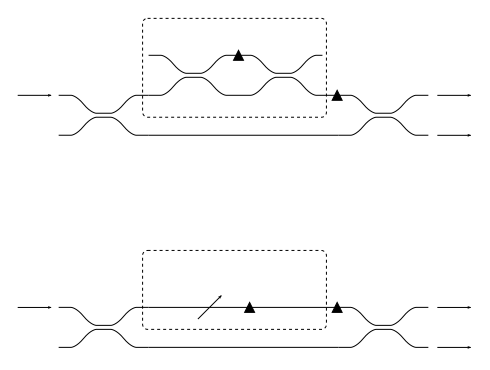
\includegraphics{figures/crosstalk}
  \caption[Nested Mach Zehnder interferometers]
  {Nested Mach Zehnder interferometers. The phase \(\theta\) controlling the
  inner MZI affects both the visibility and the origin of the fringes in the
  outer MZI. We cannot treat the phases and the reflectivities as independent.}
  \label{fig:nestedMZI}
\end{figure}

\begin{figure}[t]
  \centering
  \begin{subfigure}{\textwidth}
    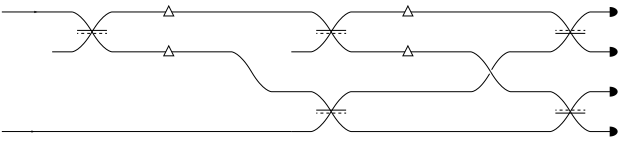
\includegraphics{figures/schematic.pdf}
    \caption{A schematic of the circuit, expanded into path}
    \label{fig:schematic}
  \end{subfigure} \\
  \vspace{1cm}
  \begin{subfigure}{0.45\textwidth}
    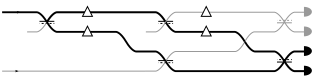
\includegraphics{figures/interferometerAB.pdf}
    \caption{A/B interferometer}
    \label{fig:ab}
  \end{subfigure}
  \hspace{0.05\textwidth}
  \begin{subfigure}{0.45\textwidth}
    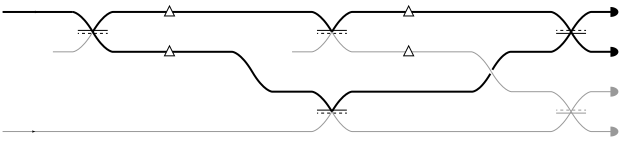
\includegraphics{figures/interferometerCD.pdf}
    \caption{C/D interferometer}
    \label{fig:cd}
  \end{subfigure}
  \caption[Illustration of nested interferometers in the bulk Reck scheme]
  {Interferometers}
  \label{fig:interferometers}
\end{figure}

\begin{figure}[t]
  \centering
  \includegraphics{figures/crapusoid}
  \caption[Interference fringes distorted by crosstalk between components]
  {Interference fringes observed in the bulk optics circuit. The distortion of
  the fringes is not due to an imperfect waveplate implementing the phase shift,
  but a kind of crosstalk between components. In this instance, the circuit
  parameters were set to \(t_{0}=22.5\deg\), \(t_{1}=24.45\deg\),
  \(q_{0}=20.95\deg\), \(q_{1}=22.5\deg\), \(q_{2}=22.5\deg\). The waveplate
  controlling \(\phi_{0}\) was fixed and the waveplate controlling \(\phi_{2}\)
  was scanned for a full rotation.}
  \label{fig:crapusoid}
\end{figure}

\section{Randomised benchmarking}
\label{sec:Benchmarking}
\begin{figure}[t]
  \includegraphics{figures/benchmarking}
  \caption[Sample data from randomised benchmarking]
  {Data from a single instance of a unitary matrix used for randomised
  benchmarking. (a) quantum coincidences; (b) classical coincidences; (c)
  singles from the `quart'; (d) singles from the `trit'. The bars show results 
  expected from theory, with the middle line being the ideal case, and the lower
  and upper lines represnting \(\pm 1\sigma\) deviations caused by errors in
  setting parameters. The points are the experimentally measured results. Error
  bars due to Poissonian noise are too small to see on this scale. The overall
  fidelity (trace distance between ideal and reconstructed matrices) is \(0.99\)
  and the fidelities of individual distributions above (Kolmogorov distance
  between normalised probability distributions) are (a) \(0.97\); (b) \(0.94\);
  (c) \(0.99\); (d) \(0.89\).}
  \label{fig:benchmarking}
\end{figure}
In order to test the calibration of the bulk optics circuit, we used it to
implement a series of Haar random unitaries: a process known as randomised
benchmarking. This testing procedure (also seen, for example,
in~\cite{peteschip}) is popular when the device being tested exhibits a high
degree of reconfigurability. By taking random samples throughout the entire
parameter space, we gain a degree of confidence that the device will work well
in any configuration. The drawback of the procedure (as I describe with a
specific example in chapter~\ref{ch:Simulations}) is that there can be small
regions of the configuration space where the device consistently
underperforms, which are unlikely to be detected by the randomised benchmarking.

I took all the data presented in this section, and performed the analysis.

The data taken consist of single photon detection statistics and two photon
correlations. For the single photon data, we can inject in two possible input
modes, and measure in four outputs (A, B, C, D), giving us two probability
distributions, each of four elements. I refer to these as the \emph{quart}
and \emph{trit} distributions, with the elements \(\vec{q}= \left( q_{A}, q_{B},
q_{C}, q_{D} \right)\) and \(\vec{t} = \left( t_{A}, t_{B}, t_{C}, t_{D}
\right)\) respectively. Subscripts refer to the detector label. Coincidences are
counted between all pairs of detectors (AB, AC, AD, BC, BD, CD), but here there
is only one input configuration. However, a delay can be introduced between
the two photons, giving us two possible probability distributions each with six
elements, which I refer to as quantum (\(\vec{Q}\)) for no temporal delay and
classical (\(\vec{C}\)) for a large temporal delay. Since the detectors are not
number resolving, we cannot measure the two photon events with multiple
occupancy, so these distributions are not normalised. An comparison of the
measured distributions to the expected distributions is illustrated in
figure~\ref{fig:benchmarking} for a single random matrix.

To assess the performance of the circuit, we consider several fidelity measures.
First, we can take the four distributions described above, \(\vec{q}\),
\(\vec{t}\), \(\vec{Q}\) and \(\vec{C}\) and compare them to the expected
distributions using the Kolmogorov distance:
\begin{equation}
  \Delta \of{ p,p^{\prime} } = \frac{1}{2} \sum_{i} \abs{p_{i} - p_{i}^{\prime}}
\end{equation}
This measure is only applicable to properly normalised distributions, so we
normalise the partial distributions \(\vec{Q}\) and \(\vec{C}\) to one for this
calculation.

The other distance measure is the trace distance between the intended unitary,
\(\mat{U}\), and the unitary that was actually applied, \(\mat{U}^{\prime}\).
The unitary that was applied is estimated from the measurements described, plus
measurements of the relative efficiency of the four detectors. The trace
distance that we use is:
\begin{equation}
  \frac{1}{2} \Tr \of{ \mat{U}^{\dagger} \mat{U}^{\prime} }
\end{equation}
where the factor of \(2\) is required because only two columns of the unitary
are considered.

The mean and standard deviations of each of these measures over the 12 random
unitaries are summarised below:
\begin{itemize}
  \item Trace distance \(0.991\pm0.015\)
  \item Quart fidelity \(0.979\pm0.005\)
  \item Trit fidelity \(0.96\pm0.03\)
  \item Quantum fidelity \(0.959\pm0.013\)
  \item Classical fidelity \(0.971\pm0.015\)
\end{itemize}


\section{Verification}
\label{sec:Verification}
Work relating to verification in quantum walks and \bosonsampling{}. I don't
think it's unfair to say that I had the original motivation to implement the
\(\rstar\) protocol described in \cite{notuniform}. I did the Bayesian model
comparison between \bosonsampling{} and uniform distributions.

Verifying the output of a Boson sampler brings us up against the notorious
problem of certifying a random number generator based on a short string of
random output. This problem is illustrated in figure:~\ref{fig:dilbert}

\subsection{Is BosonSampling uniform?}
\label{sec:RStar}
\begin{figure}[t]
  \centering
  \includegraphics[width=\textwidth]{figures/protected/dilbert.png}
  \caption[Dilbert discovers that verifying randomness is difficult.]
  {Dilbert discovers that verifying randomness is difficult.\\DILBERT
  \textcopyright{} 2001 Scott Adams. Used By permission of UNIVERSAL UCLICK. All
  rights reserved.}
  \label{fig:dilbert}
\end{figure}

\begin{figure}[t]
  \centering
  \includegraphics{figures/rstar}
  \caption[Using the $\rstar$ discriminator to verify BosonSampling]
  {(a) Expected distribution of \(\rstar\) values when events are sampled
  uniformly (black) and from the full quantum distribution (blue). Experimental
  data from a 3-photon experiment in a 9-mode unitary is shown as a histogram.
  (b) Bayesian model comparison allows real-time updating of our confidence in
  the model describing our data. The models under comparison here are true
  \bosonsampling{} (blue) and uniform sampling (black). We rapidly conclude that
  the data are supported much better by the \bosonsampling{} model.}
\end{figure}

\subsection{Bosonic Clouding}
\label{sec:Clouding}
\begin{figure}[t]
  \centering
  \includegraphics{figures/clouds}
  \caption[Bosonic clouding in a quantum walk]
  {Simulation and experiment for a 21-mode, 3-photon quantum walk, showing the
  phenomenon of bosonic clouding. In all plots a sphere is drawn for every
  possible detection event. The indices of the output modes dictate the
  position, so for the event where the photons are detected in modes \(i\),
  \(j\) and \(k\), a sphere will be drawn at \(\left(i,j,k\right)\) on these
  axes. The size of the sphere indicates the probability of the event occuring. 
  The clustering of events around but not necessarily on the line \(i=j=k\)
  (drawn in black) is the phenomenon that we call bosonic clouding.
  (a) and (b) show simulations of the quantum walk; (c) and (d) show the
  experimental data; (a) and (c) (blue) are quantum data, i.e. indistinguishable
  photons; (b) and (d) (red) are classical i.e. photons made distinguishable by
  introducing a time delay.\\
  (Plots by Pete Shadbolt, used with permission.)}
\end{figure}
In a multi-photon quantum walk, we observe a phenomenon where photons tend to
appear in nearby output modes. This is distinct from \emph{Bosonic bunching},
where multiple photons appear in the same output mode.

\subsection{Higher photon numbers}
\label{sec:SixPhoton}
\begin{figure}[t]
  \centering
  \includegraphics{figures/sixphoton}
  \caption[Bayesian model comparison on 6-photon events]
  {Bayesian model comparison using the full pre-calculated 6-photon
  distributions. (a) Events we believe to be quantum. (b) Events we believe to
  be classical. In both cases, our confidence in the model quickly increases.}
  \label{fig:sixphoton}
\end{figure}
I did some verification on 6-photon events in the recent integrated Reck
experiment. With the circuit set to implement the 6-dimensional quantum Fourier
transform, we injected 6 photons in the state \(\ket{3_{1},3_{2}}\) and
performed a Bayesian model comparison between the quantum and classical
distributions. Again, we quickly become very confident that the data are
quantum, as shown in figure~\ref{fig:sixphoton}.

It's worth mentioning somehow that the quantum interference here is in some way
not `true' 6-photon quantum interference. It seems to come out as equivalent to
around 3 photons, but I can't remember quite how Chris and I came up with that
figure.

The photons are injected into just two input modes. In order to obtain classical
results, it is sufficient to introduce a time delay between these two modes,
without applying relative delays between the three photons in the same mode.
This is readily derived by considering the probabilities of output events in
terms of matrix permanents.
